Our first preprocessing approach produces pictures that are well-readable and understandable for humans. We were concerned however how well they can work with convolutional layers. The reason for our scepticism was that on real pictures the pixels tend to highly correlate with the other pixels in their surroundings. This can not be said about our preprocessing, which contains sudden changes. We implemented another method using Hilbert’s curves. In a nuttshell: Hilbert’s curves~\cite{hilbert} is a way to map the 1Darray-like amplitudes of a song (which are stored by many music file) to a 2D picture, in such way, that the notes close to each other in the array will also be close on the 2D picture. This approach might work better with convolutional networks since the small kernels, parsing the picture can actually extract features that correlates more.

\subsubsection{Encoding}
The encoding was done by a rather simple, custom written, recursive (because of the recursive nature of Hilbert's curves) function, that expects a $4^x$ number of samples. Divides them equally into four groups and calls itself with each group, then places the resulting  $4$ matrices to their corresponding position, while rotating and mirroring the bottom $2$.

%\ref{fig:hilbert}
\begin{figure}[H]
	\centering
	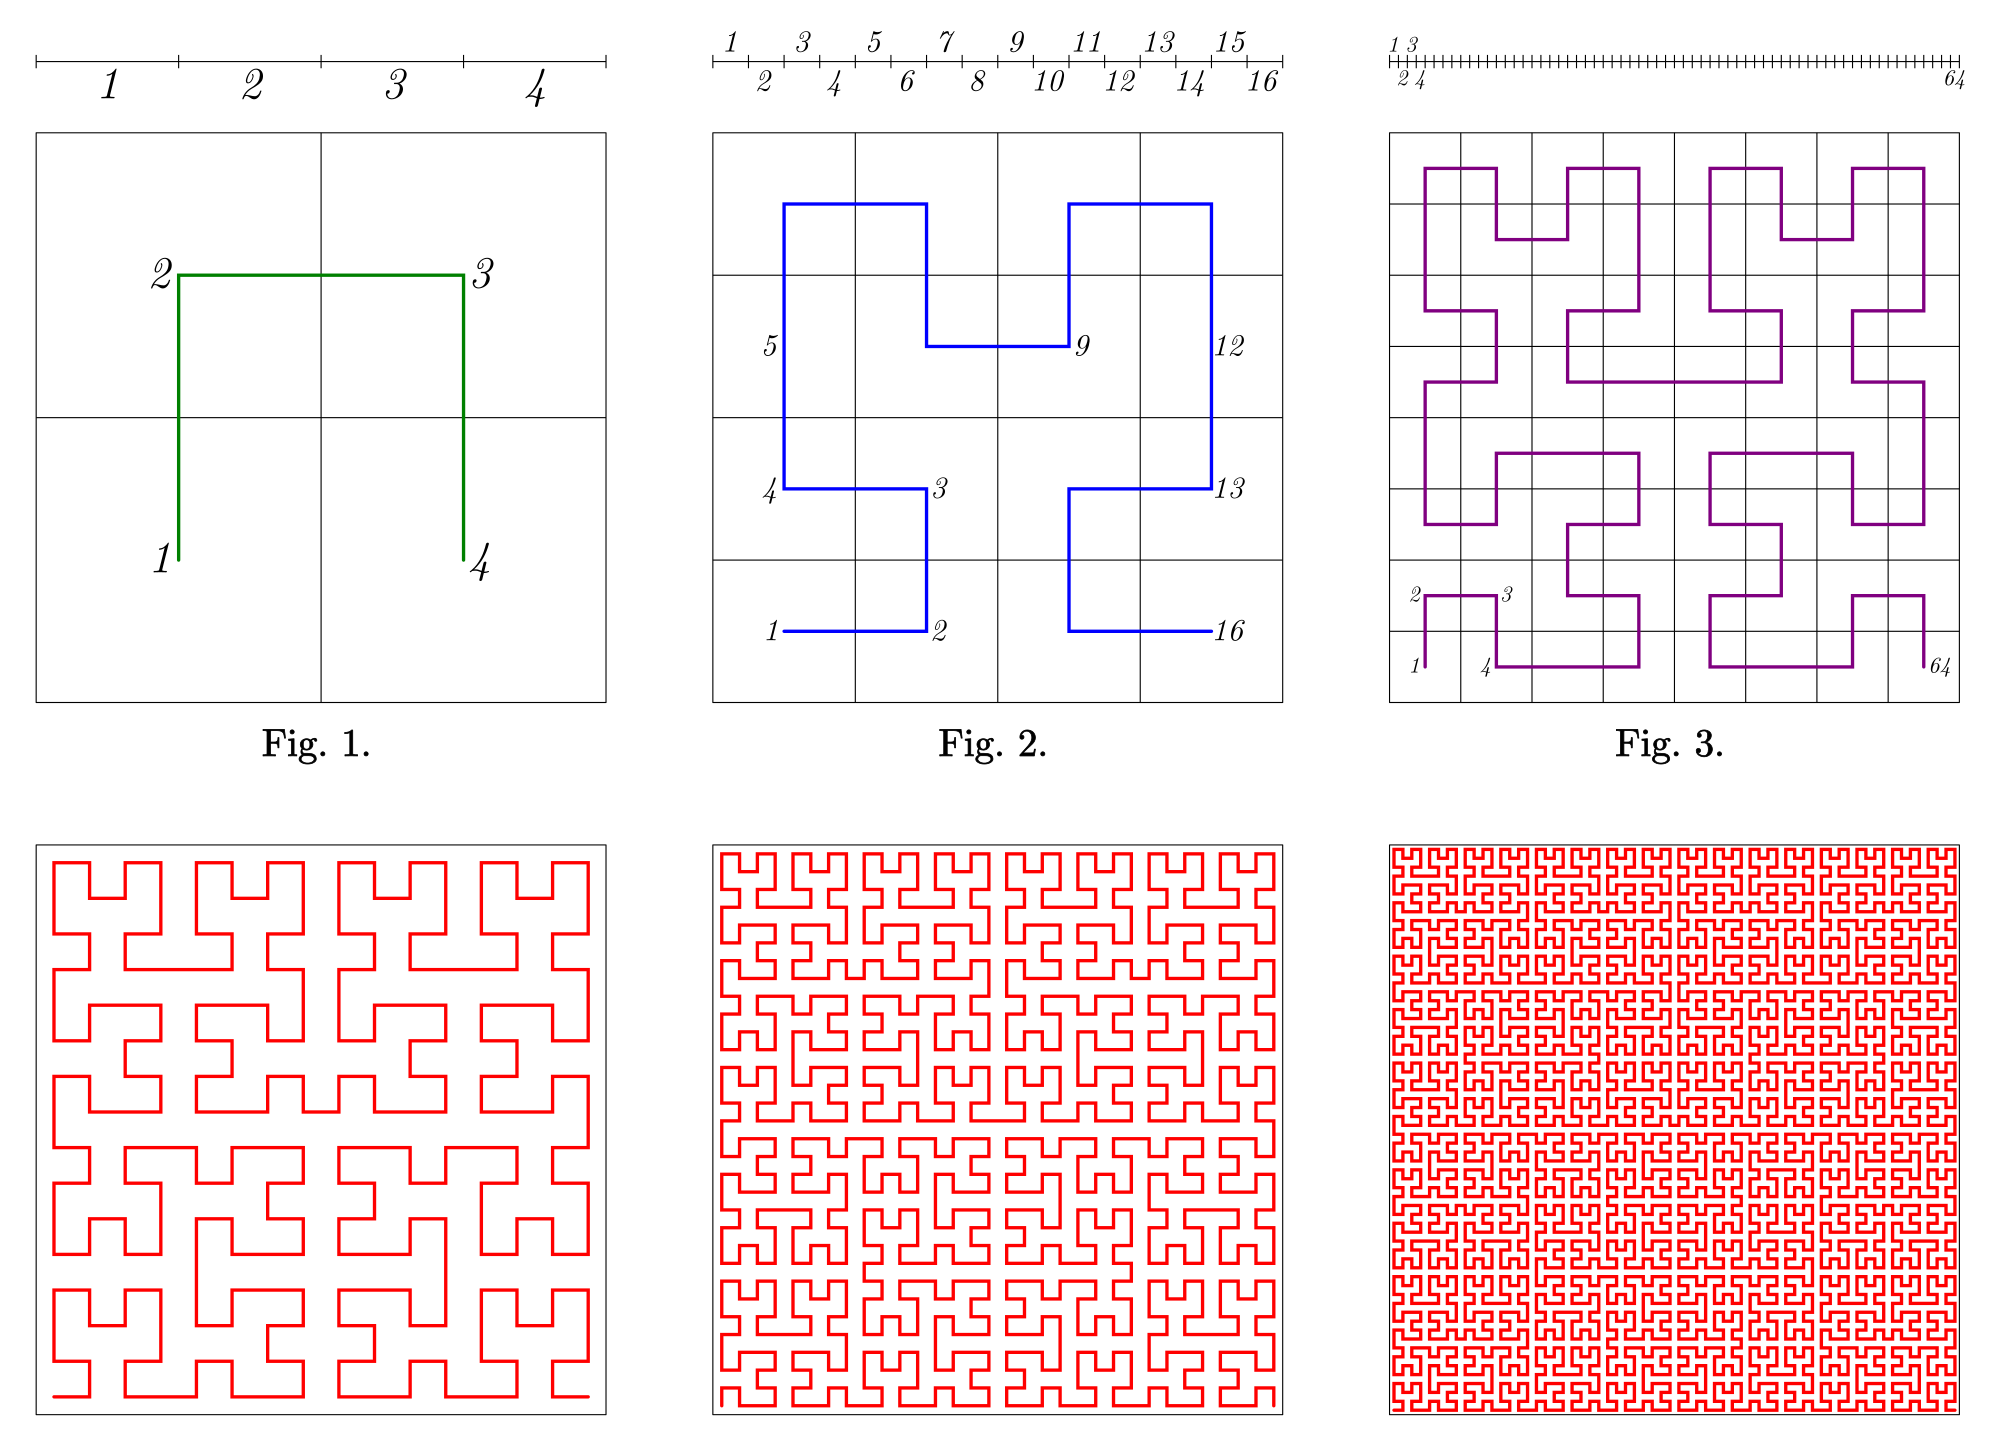
\includegraphics[width=\linewidth]{hilbert.png}
	\caption{Construction of more and more complex Hilbert curves.}
	\label{fig:hilbert}
\end{figure}

Obviously this approach does not work properly with the .midi files, thus we had to use their .wav version ($44100$Hz sampling rate, $2$ channels and $16$ bit values). We decided to use $256*256$ one channeled pictures (well technically they are not pictures but arrays). This means that on $1$ picture we can store $256*256/44100 = 1.49$ second long music. Might be worth adding, that we also scaled the resulting "pictures" to be between 0 and 1.

\subsubsection{Decoding}
The decoding is done by reversing the encoding. After it is done, we can write the 1D array into a .wav file and listen to the result.